\chapter{算法分析及系统架构设计}
本章将针对循环神经网络前向传播过程提出一套从软件算法,硬件实现到系统集成的全流程设计框架和独立整的解决方案。不同于所有过往的压缩加速设计,
本文所采用的压缩算法具有压缩成本小,无需训练集等优势,可以不依赖云端算力支持,仅在分布式的边缘设备实现,算法的详细介绍将在3.1节展开。算法特性
决定了其适用场景,而具有弹性性能需求的应用场景又是普遍存在的,所以在现实条件的约束下,本文对算法进行了合理的拆分与协同并分别映射到软件和硬件上
进行执行,具体的系统架构设计见3.2节。最后,面向算法和应用场景需求,本文进行了定制化专用硬件架构的设计,通过对上层应用的需求和硬件加速空间
进行分析,本文创造性的提出了一种具有紧凑计算结构和可配置功能模块的循环神经网络前向传播硬件加速器。该加速器能通过简单的配置和数据重载完成不同网络结构
和不同模型大小的切换,相比传统的神经网络加速器的一种硬件实现对应唯一的网络结构和模型尺寸,本文所设计的加速器即具有“专用”所带来的高效性,
又具有一定程度“通用”所带来的灵活性,能满足弹性应用场景下性能可调的需求。在众多的循环神经网络模型中,本文选取回声状态网络作为设计实例,因其结构简单,
训练成本低和应用前景开阔等优势,同时又极具代表性和紧迫性,详细分析说明可见2.1节。对于其他种类的循环神经网络,除具体实现细节存在微小差异外,本文在
系统层面提出的设计方案,软件算法和硬件架构设计也同样适用,因此,本文不再一一说明。
\section{基于投影的模型压缩算法}
本小节先展示模型压缩的效果---简化网络结构,然后就简化网络的生成过程(状态投影和激活函数近似)作详细的说明,最后会评估与分析压缩算法的特性和作用效果。
以上描述的模型压缩的全景图是本文后续工作的基础。
\subsection{简化网络结构}
回声状态网络在模型压缩算法的作用下生成了简化网络,其数学模型为式\ref{eq:redesn},式中\(\widehat{x},\widehat{z} \in \mathbb{R}^q\)表示简化网络隐藏层的状态,
\(\widehat{W}, \widehat{E}_d \in \mathbb{R}^{q \times q}\)表示隐藏层与隐藏层的连接权重,\(\widehat{E}_l,\in \mathbb{R}^{q \times q}\)表示隐藏层跨时间步的自循环矩阵,
\(\widehat{W}_{in},\widehat{W}_{out}\in \mathbb{R}^{q \times n_{in}}\)分别表示输入到隐藏层以及隐藏层到输出的连接权重,\(q\)是隐藏层的神经元数量,
\(n_{in}\)为输入数量,\(n_{out}\)为输出数量。
\begin{equation}\label{eq:redesn}
	\begin{split}
		\widehat{z}_t &= f(\widehat{W} * \widehat{x}_{t-1} + \widehat{W}_{in} * u_{t})				\\	
		\widehat{x}_t &= \widehat{E}_l * \widehat{x}_{t-1} + \widehat{E}_d * \widehat{z}_{t} 		\\
		y_{t} 			&= \widehat{W}_{out} * \widehat{x}_{t}	
	\end{split}
\end{equation}

相较于回声状态网络的原网络模型,简化网络的数学描述更加复杂, 具体表现为引入了新的状态变量\(\widehat{z}\)和新的新的拓扑连接\(\widehat{E}_l,\widehat{E}_d\)。
\(\widehat{z}\)是输入\(u\)和状态\(\widehat{x}\)的函数,而\(\widehat{x}\)又与暂态\(\widehat{z}\)呈线性相关的关系。这些新引入的变量和关系
改变了回声状态网络的模型结构,即简化网络在原网络结构的基础上增加了一层隐藏层,如图\ref{fig:esn_convert}所示。此外,简化网络拥有两个循环结构:暂态\(\widehat{z}\)
和状态\(\widehat{x}\)之间的层间循环体和状态层\(\widehat{x}\)内部的自循环体。循环体的增加赋予了循环神经网络更强大的记忆能力,这使得少量的隐藏层神经元
就可以实现对系统动态特性的表征。显然,本文所采用的模型压缩算法在网络结构上做出了让步,但是“祸兮,福之所倚”,简化网络在压缩神经元数量方面取得了巨大的成功。
二者利害相权的最终结果是:在模型预测精度不显著下降的情况下,简化网络的参数量将大幅减少,前向传播过程的时间复杂度也显著降低。
\begin{figure}
	\centering
	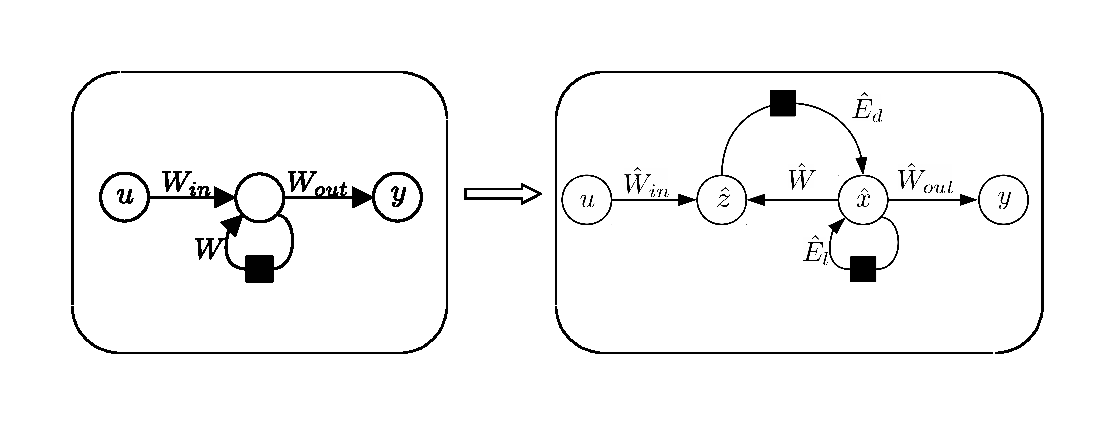
\includegraphics[width=0.7\columnwidth]{ESN_convert.eps}
	\caption{原始网络和简化网络的结构图}
	\label{fig:esn_convert}
\end{figure}

简化回声状态网络的结构如图\ref{fig:esn_red}所示。该网络的深度为四,包括输入层\(u\),输出层\(y\)和两层隐藏层\(\widehat{z},\widehat{x}\)。
其中输入层,输出层和状态层\(\widehat{x}\)保留了原网络相似的结构和映射关系。暂态\(\widehat{z}\)是新引入的结构,其作用在于桥接输入层和状态层,
对流经该层的信息做初步的加工处理。暂态层\(\widehat{z}\)和状态层\(\widehat{x}\)共同组成隐藏层,数据在两层隐藏层之间双向流动,形成一个大的信息回路。
但是两层隐藏层也存在差异,暂态层不存在自循环体,因此传统上意义上不能称为状态,考虑到其也位于数据循环的关键路径,因此称之为暂态。实际上
仅从结构特性而言,暂态层和全连接层有更大的相似度。以上分析了简化网络的结构特性,相较于原网络,既存在保留部分,也添加了新的元素。 

\begin{figure}
	\centering
	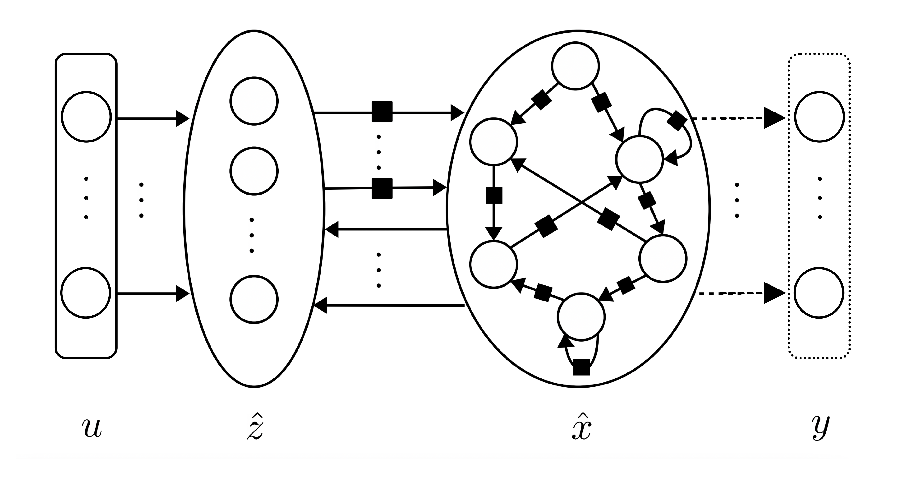
\includegraphics[width=0.7\columnwidth]{ESN_red.eps}
	\caption{简化回声状态网络结构}
	\label{fig:esn_red}
\end{figure}

简化网络的前向传播速度相较原网络会大幅提升,这得益于隐藏层神经元数量的减少。简化网络内部神经元的数量每层\(q\)个,远小于原网络的\(n\)个。
相应的,网络中神经元的连接复杂度也将降低,权重矩阵的参数量将从\(n^2\)变为\(q^2\)。以上神经元数量和权重参数量的压缩将会直观的反映到模型的
计算复杂度上,原网络每个时间步长的前向传播计算复杂度为
\begin{equation}
	\mathcal{O}(n^2 + n*n_{in} + n*n_{out})
\end{equation}
简化网络的前向传播计算复杂度为
\begin{equation}
	\mathcal{O}(q^2 + q*n_{in} + q*n_{out})
\end{equation}
在输入输出数量不变的条件下,简化网络的时间复杂度仅由\(q\)决定,和原网络的阶数\(n\)无关。又因为\(q<<n\),所以简化网络前向传播的速度会比原网络快很多。
具体的\(q\)值的选取需根据用户对精度和速度的需求来确定,简化网络的阶数\(q\)越小,模型的计算速度越快;\(q\)越大,模型的精度越高。

\subsection{网络压缩}
前面的叙述介绍了简化回声状态网络和原网络之间在网络结构上的相似性和差异性,解释了简化网络模型预测精度不会显著下降的原因,并从计算复杂度的角度说明了
简化网络在前向传播过程中加速能力的来源,下面本小节将就原网络如何生成简化网络进行简要的说明,模型压缩算法的具体推导请见文献\citing{WangLong:TNNLS'23}。
%介绍高速回声状态网络的生成,算法顺序介绍,or硬件需求倒推
\subsubsection{基于投影的状态近似}
为了记忆动态系统丰富的时序特性,循环神经网络一般拥有庞大数量的隐藏层神经元,这些神经元互连关系复杂,对信息拥有记忆和遗忘功能,是循环神经
网络最重要的组成部分。对于简单的任务,仅需要少量的神经元便可完成,而复杂的任务则需要更多神经元协同。实际情况下,任务的复杂程度判别具有
相当程度的主观性,隐藏层神经元数量会被保守的设置为远超实际需求的数量,即存在大量的冗余性。本小节针对神经元的冗余性,采用基于投影的状态近似方法进行消除。
状态近似框架:
\begin{equation}
	V_x * \widehat{x}_{t} \approx x_{t}
\end{equation}
其中\(V_x \in \mathbb{R}^{n \times q}\)是投影矩阵,满足\(V_x^T * V_x = I\),\(x_{t} \in \mathbb{R}^n\)是状态向量,\(\widehat{x}_t \in \mathbb{R}^q\)是状态近似向量。
状态近似将高维向量\(x_t\)投影到状态空间中,并用状态空间的基向量进行线性表示,其坐标为\(\widehat{x}\)。实际上,由于输出只需要选择性的保留
动态系统过去序列的某些方面信息,而与其他方面无关,系统的动态特征往往有限且集中。这在状态空间上表现为:和任务输入输出相关的状态只占全部状态的一部分,即
有效状态空间是满状态空间的子空间。按照状态子空间中特征的重要程度划分,有效状态空间又可以分为核心特性空间和外围特征空间。在进行状态投影时,状态向量将首先
被投影到核心特征空间中,在这种状态近似情况下,模型的预测不会偏离真实输出太大;其次,状态将会被投影到外围特征空间,该空间越大,模型就越能捕捉系统微小
的动态特征,模型的输出也就越具有丰富性。状态子空间的选取将会对状态近似后的网络预测效果产生较大的影响,如何构造状态空间以实现较好的近似将在3.1.2.3中介绍。\\
将状态近似代入回声状态网络模型\ref{eq:esn}得到
\begin{equation}
	\begin{split}
		\widehat{x}_{t} & = V_x^T * f(W*V_x * \widehat{x}_{t-1} + W_{in} * u_t)	\\
					y_t & = W_{out} *V_x * \widehat{x}_t
	\end{split}
\end{equation}
基于投影的状态近似方法生成的简化网络除了隐藏层神经元数量更少以外,还在自循环结构上增加了线性算子。该算子需要在状态激活后
作用于每一个隐藏层神经元,并且运算次数为\(n\),这导致隐藏层的等效神经元数量也为\(n\)。为了获取真正的模型简化,一个直观的想法是将\(V_x^T\)
移动到激活函数内部,形成类似\(V_x^T * W * V_x\)的\(q \times q\)矩阵,这样模型压缩后等效神经元的数量也为\(q\),简化网络前向传播的时间复杂度
也将进一步降低。然而循环神经网络的激活函数通常是非线性的,非线性算子和线性算子的顺序是不能更改的,这个想法无法直接实现。


选择矩阵

\subsection{压缩算法的评估与析}
从精度和复杂度方面分析。

\section{系统整体架构设计}
应用场景介绍引入软硬件功能划分。
\subsection{前向传播及压缩流程}
\subsection{软硬件功能划分}
\subsection{系统整体架构}

\section{面向算法的定制化硬件分析}
\subsection{算法需求分析}
1需要实现原始网络,高速网络两个网络结构。
2压缩网络结构尺寸可调节。
3模型压缩过程。
\subsection{硬件模块划分与复用性分析}
\subsection{激活函数分段近似}
\subsection{计算资源与存储资源需求分析}

\section{基于FPGA的加速器设计}
\subsection{硬件加速器整体架构}

\subsection{存储架构设计}

\subsection{计算架构设计}

\subsection{矩阵向量乘法模块}

\subsection{激活函数模块}

\subsection{IP核互联设计}

\section{本章小结}
